\documentclass{article}
\usepackage[utf8]{inputenc}
\usepackage{graphicx}
\usepackage{listings}
\title{Information System - Lab work 8}
\author{Tran Thi Hong Hanh}
\date{10 November 2017}

\begin{document}

\maketitle
\section{Requirement}
You need a database to manage information about the magazines that you buy habitually.\\
For each magazine, its title, the ISSN (code that identifies the publication), number and year are stored. You need also data about the articles, including its title, page of beginning and page of ending. It is assumed that there are no two articles with the same title.\\
Every article can be written by several authors, whose name, e-mail address and ascription are stored. Besides, a number that indicates the order of has to be stored.
\section{Design Database}
\subsection{Determine concepts that needs to be stored}
\begin{itemize}
	\item Magazine
	\item Article
	\item Author
\begin{figure}[h]
\centering

\includegraphics[scale = 1]{1.PNG}
\caption{Concepts}
\end{figure}
\end{itemize}
\subsection{Determine attributes of each concept}
\begin{itemize}
	\item Magazine (title, ISSN, number, year, order\_no)
	\item Article (title, begin\_page, end\_page) 
	\item Author (name, email, ascription)
\begin{figure}[h]
\centering
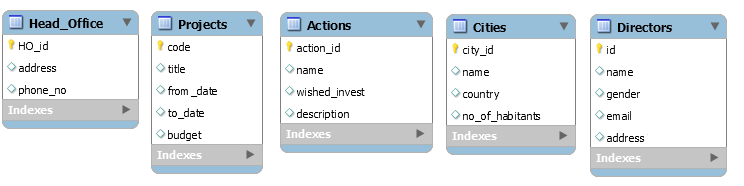
\includegraphics[scale = 1]{2.PNG}
\caption{Attributes}
\end{figure}
\end{itemize}

\subsection{Determine links (relationships) between them}
\begin{itemize}
	\item Article and Magazine ("has")
	\item Article and Author ("has")
\end{itemize}
\subsection{Determine types of each concept attribute}
\begin{itemize}
	\item Magazine 
	\begin{itemize}
	\item title VARCHAR(100)
	\item ISSN VARCHAR(20)
	\item number INT
	\item year INT
	\item order\_no INT
	\end{itemize}
	\item Article 
	\begin{itemize}
	\item title VARCHAR(100)
	\item begin\_page INT
	\item end\_page INT
	\end{itemize} 
	\item Author 
	\begin{itemize}
	\item name VARCHAR(50)
	\item email VARCHAR (50)
	\item ascription VARCHAR (200)
	\end{itemize} 
\begin{figure}[h]
\centering
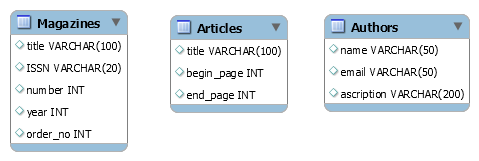
\includegraphics[scale = 0.7]{3.PNG}
\caption{Type of attributes}
\end{figure}
\end{itemize}

\subsection{Solve foreign key links}
\begin{itemize}
	\item Magazines 
	\begin{itemize}
	\item magazine\_id INT
	\item title VARCHAR(100)
	\item ISSN VARCHAR(20)
	\item number INT
	\item year INT
	\item order\_no INT
	\end{itemize}
	\item Articles 
	\begin{itemize}
	\item article\_id INT
	\item title VARCHAR(100)
	\item begin\_page INT
	\item end\_page INT
	\item magazin\_id INT
	\end{itemize} 
	\item Authors 
	\begin{itemize}
	\item author\_id INT
	\item name VARCHAR(50)
	\item email VARCHAR (50)
	\item ascription VARCHAR (200)
	\end{itemize}
	\item Article\_Author
	\begin{itemize}
	\item article\_id INT
	\item author\_id INT
	\end{itemize}	 
\begin{figure}[h]
\centering
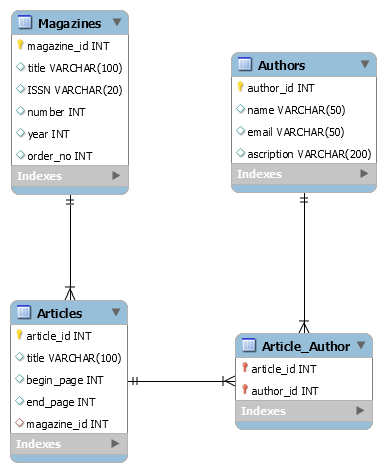
\includegraphics[scale = 0.7]{4.PNG}
\caption{Solve foreign key links}
\end{figure}
\end{itemize}
\newpage
\subsection{Implementation}
\begin{lstlisting}{showstringspaces=false}[language=SQL]
CREATE DATABASE Magazines;
USE Magazines;

CREATE TABLE Magazines (
  magazine_id INT NOT NULL,
  title VARCHAR(100),
  ISSN VARCHAR(20),
  number INT,
  year INT,
  order_no INT,
  PRIMARY KEY (magazine_id)
 );
  
CREATE TABLE Articles (
  article_id INT NOT NULL,
  title VARCHAR(100),
  begin_page INT,
  end_page INT,
  magazine_id INT,
  PRIMARY KEY (article_id),
  FOREIGN KEY (magazine_id)
  REFERENCES Magazines(magazine_id)
);

CREATE TABLE Authors (
  author_id INT NOT NULL,
  name VARCHAR(50),
  email VARCHAR(50),
  ascription VARCHAR(200),
  PRIMARY KEY (author_id)
);
  
CREATE TABLE Article_Author (
  article_id INT NOT NULL,
  author_id INT NOT NULL,
  PRIMARY KEY (article_id, author_id),
  FOREIGN KEY (article_id) REFERENCES Articles(article_id),
  FOREIGN KEY (author_id) REFERENCES Authors(author_id)
 )
    
\end{lstlisting}
\begin{figure}[h]
\centering
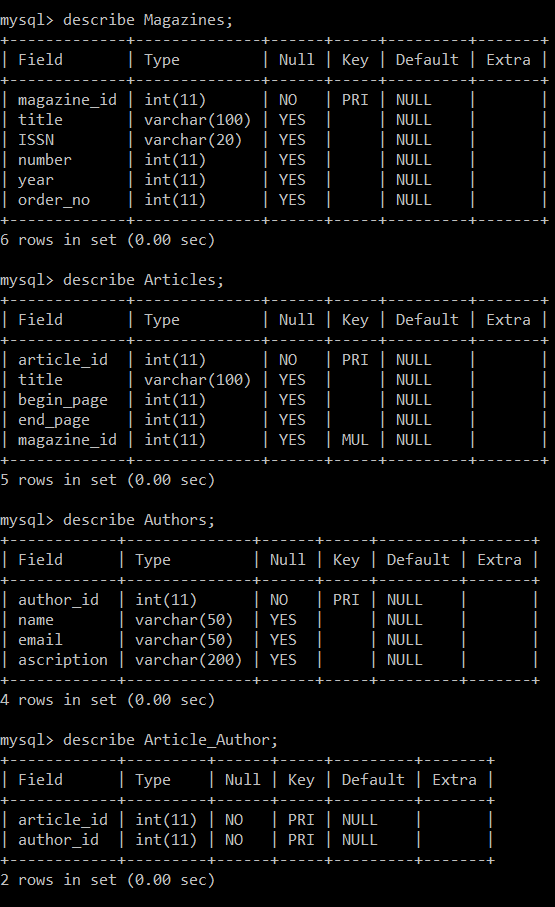
\includegraphics[scale = 0.7]{5.PNG}
\caption{Output}
\end{figure}

\end{document}
